\documentclass[12pt,letterpaper,USenglish]{article}

\usepackage[most]{tcolorbox}
\usepackage{amsmath}
\usepackage{amssymb}
\usepackage{microtype}
\usepackage{tikz}
\usepackage{paralist}
\usetikzlibrary{calc,positioning,backgrounds,intersections,graphdrawing,shapes,graphs,arrows}
\usegdlibrary{trees}

%%% Please use define.org for macros.
\input{define.orgtex}

\begin{document}

\makeatletter
\tikzset{use path/.code=\tikz@addmode{\pgfsyssoftpath@setcurrentpath#1}}
\makeatother
\tikzset{lead/.style={anchor=north west,font=\it\bfseries,text=algs4red},
    graphs/mytree/.style= {
    tree layout, minimum number of children=2,
    sibling distance=5mm, level distance=5mm,
    nodes={draw, minimum
      height=13pt, fill=white,inner sep=2pt, font=\footnotesize,
      rounded rectangle},
    edges={thick}}}

\noindent\begin{tikzpicture}[every node/.style={anchor=north west}]
  % Main background
  \begin{scope}[on background layer]
    \fill[black!10!white, draw=white, line width=6pt] (-.5\textwidth, 0) rectangle (.5\textwidth, -18cm);
  \end{scope}

  % Clip and left margin
  \path [save path=\theframe, rounded corners] ($(-.5\textwidth, 0) + (1.5pt,-1.5pt)$)
                rectangle ($(.5\textwidth, -18cm) + (-1.5pt, 1.5pt)$);
  \clip [use path=\theframe];
  \coordinate (left) at ($(-.5\textwidth, 0) + (0.3cm,0)$);

  % Title
  \node [anchor=north,text width=20cm,minimum height=1.4cm,align=center,fill=algs4red,text=white]
  {\sffamily\Large \textbf{3.3}\quad BALANCED SEARCH TREES: 2-3 TREES};

  % Definition
  \node [lead] (def) at (left |- 0, -1.6cm) {Definition.};
  \node [right=0cm of def.north east, anchor=north west] {%
    \begin{minsizebox}{.8\textwidth}{10cm}
      A \emph{balanced} tree of 2- and 3-nodes.  A 2-node is a node with one key
      \(k\) and two subtrees; the keys in the left subtree are smaller than
      \(k\), the keys in the right subtree are greater than \(k\).  A 3-node is a
      node with two keys \(k < k'\) and three subtrees; the keys in the left
      subtree are smaller than \(k\), the keys in the middle subtree are between
      \(k\) and \(k'\), the keys in the right subtree are greater than \(k'\).
    \end{minsizebox}%
    };

    
  % Example
  \begin{scope}[shift={($(def.south west) + (0cm,-2.4cm)$)},
    every node/.style={anchor=south},
    note/.style={font=\footnotesize},
    edgenote/.style={algs4red,->,>=stealth',shorten >=3pt}]
    % Background & lead
    \begin{scope}[on background layer]
      \fill[black!15] (-0.07, 0.35) rectangle (19.05, -3.2);
    \end{scope}
    \node[lead,draw=none,shape=rectangle] at (0, 0.3) {Example.};

    \graph [mytree] { 7 [x = 3cm,y=-0.6cm] -- { 35 [as={3~~5}] -- {1 2, 4, 6}, {9 -- {8,
            11 12}}} };
    \begin{scope}[on background layer]
      % \node[draw=algs4red, fill=algs4red!20, thick,anchor=center,circle,minimum
      % width=20pt] (c) at (4) {};
      \path[draw=algs4red, fill=algs4red!20, thick] (35.center) -- ($(4.center) +
      (-200:10pt)$) arc (-200:20:10pt) -- cycle;
      \node[note,anchor=center,yshift=-1cm] (n) at (4) {between 3 and 5};
      \draw ($(n.north)+(0cm,-0.1cm)$) edge [edgenote,shorten >=2mm] (4);
    \end{scope}

    \node[lead,draw=none,shape=rectangle] at (7, 0.3) {Nonexamples.};

    \graph [mytree] { 7 [x = 10.5cm,y=-0.6cm] -- { 3 -- {1, 4}, {8 -- { ,
            9}}} };
    \node[note,text width=2cm,align=center] (n) at (8cm,-2cm) {\emph{null} link not at lowest
      level};
    \draw (n.east) edge[edgenote, bend right] (8);
    
    \graph [mytree] { root [as={2~~4~~6},x = 13.5cm,y=-0.6cm] -- {1, 3, 5, 7}};
    \node[note] (n23) at (17cm,-.8cm) {not a 2- or 3-node};
    \draw ($(n23.west) + (0cm, -0cm)$) edge [edgenote,bend right] (root.east);

    \graph [mytree] { 4 [x=13.5cm, y=-2cm] -- {1, 4p [as=4], 7} };
    \draw[algs4red,thick] ($(4.south) + (0cm, 0.6cm) + (-140:.7cm)$) arc
    (-140:-40:.7cm);
    \node[note] (n) at (17cm, -2.5cm) {too many children};
    \draw (n.west) edge[edgenote,bend left] ($(4) +(.4cm,-.12cm)$);
  \end{scope}

  % Algorithms
  \node [text width=20cm, fill=algs4red,text=white, align=left] (algs) at (-.5\textwidth,-8.5cm)
  {\sffamily\bfseries ~~Algorithms};

  \begin{scope}[shift={($(left |- algs) + (0cm,-.4cm)$)}]
    \node[lead] (s) {Search.};
    \node [right=0cm of s.north east,anchor=north west] {Generalized binary
      search.};

    \node[below=0cm of s.south west,lead] (s) {Insert.};
    \node[right=0.15cm of s.north east,anchor=north west] {%
      \begin{minsizebox}{.8\textwidth}{10cm}
        Insert at leaf.\\
        \myto{} If 2-node, turn into 3-node, done.\\
        \myto{} If 3-node, turn into 4-node, then\\
        \qquad split up until no 4-node.        
      \end{minsizebox}};
    \node[fill=black!15] at (9cm, -0.1cm) {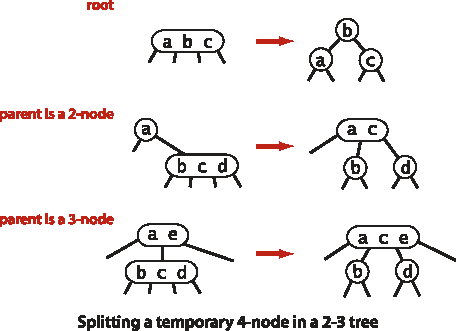
\includegraphics[height=6cm]{split}};
    
    \node[below=1.5cm of s.south west, lead] (s) {Delete.};
    \node[right=0.08cm of s.north east,anchor=north west] {%
      \begin{minsizebox}{.8\textwidth}{10cm}
        Go down the tree searching for key.\\
        Make sure current node is not 2-node,\\
        \quad by possibly introducing a 4-node.\\
        When key found, replace with successor.\\
        Continue going down to erase successor.\\
        Erase at leaf from 3- or 4-node.\\
        Go up the tree, splitting 4-nodes.
      \end{minsizebox}};
  \end{scope}
 

  % Costs
  \node [text width=20cm, fill=algs4red,text=white, align=left] (costs) at (-.5\textwidth,-16cm)
  {\sffamily\bfseries ~~Costs};
  \node [text width=.9\textwidth] at ($(left |- costs) + (0, -.1cm)$) {
    \begin{compactitem}
    \item The height of an \(N\)-key 2-3 tree is between
      \(\lfloor\log_3 N\rfloor\) (all 3-nodes) and \(\lfloor \lg N \rfloor\) (all 2-nodes).
    \item All the algorithms above run in time \(O(\lg N)\).
    \end{compactitem}
  };

  %% Box
  \draw [algs4red,line width=3pt] [use path=\theframe];

\end{tikzpicture}
\end{document}
%%% Local Variables:
%%% ispell-local-dictionary: "en_US"
%%% TeX-master: t
%%% End:
